\section{Model Based Approach}

We saw in section \ref{section:iter} that the approach is not scalable as it is expensive to run the jobs multiple times. In this section, we will propose an alternative approach of using mathematical models to recommend new settings. In earlier part of section we would present key insights that lead us to develop simple models for Big Data SQL Engines. In latter part we would discuss a model for Hive on Hadoop Map Reduce which can be used to recommend optimal settings. We would also present detailed experimental evaluation of our model.

\subsection{Key Insights}

We have run multiple experiments to optimize real world SQL workloads of our customers. This helped us to gain few key insights that we helped us to come with simple model. Following are those insights:

\noindent\subsubsection*{\bf Container shape should match that of Instance shape}
Yarn allocates containers on two dimensions - \textbf{memory} and \textbf{vcpu}. Each container is given 1 vcpu and some memory. The memory/vcpu of the containers should match the memory/vcpu ratio of the machine type. Otherwise resources are wasted. Figure \ref{fig:container_shape} illustrates three scenarios:
\begin{enumerate}[label=(\alph*)]
\item Memory/vCPU ratio of container is same as that of instance; hence, neither memory nor CPU is wasted. 
\item Memory/vCPU ratio of container is smaller than that of instance; hence, memory is wasted as extra memory of instance is still remaining unused after container allocation.
\item Memory/vCPU ratio of container is higher than that of instance; hence, CPU is wasted as extra CPU of instance is remaining unused after container allocation.
\end{enumerate}

\begin{figure*}[h]
	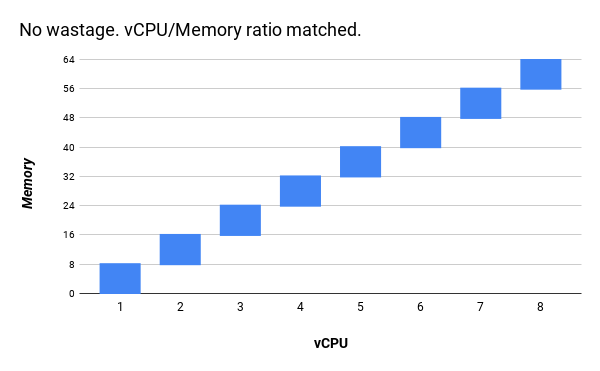
\includegraphics[width=0.33\linewidth]{container_shape1.png} 
	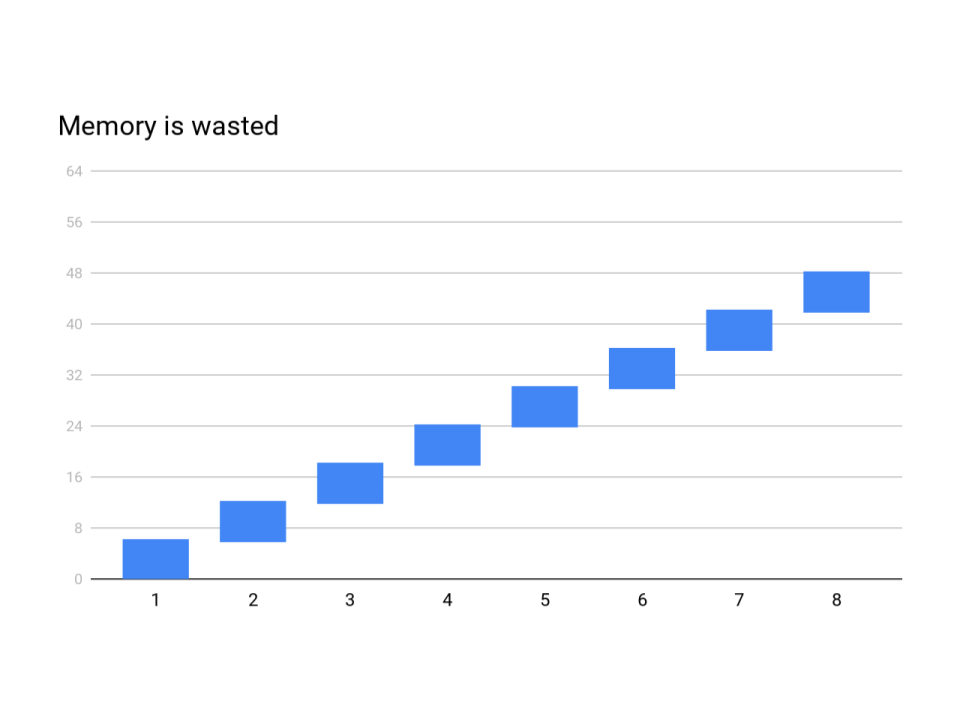
\includegraphics[width=0.33\linewidth]{container_shape2.png}
	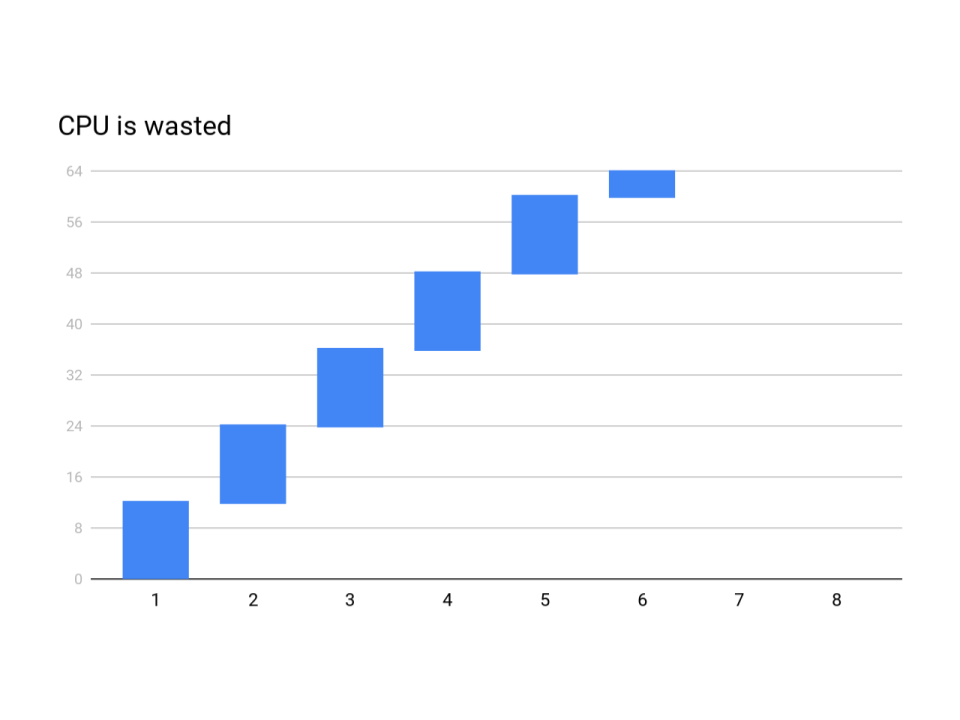
\includegraphics[width=0.33\linewidth]{container_shape3.png}
	%\vspace*{-15pt}
	\caption{\textbf{(a)} No Resource is wasted \textbf{(b)} Memory is wasted \textbf{(c)} CPU is wasted}
	\label{fig:container_shape}
\end{figure*}

\noindent\subsubsection*{\bf Avoid Data Spills at all cost}
Data Spills happen when the buffer allotted is not enough to hold data and it's written to disk. Spills are expensive because each spill leads to an extra write and read of the data. In our experiments, we have found spills to add major overhead and should be avoided at all cost. Spills can be avoided by providing adequate memory to each task or by by making more fine grained tasks.
For example in Map Reduce, mapper spills can be avoided either by increasing Mapper container size or by reducing split size so that mapper tasks would process lesser data which might avoid spill.

\noindent\subsubsection*{\bf Decrease memory per task to choose a cheaper instance type}
On cloud platforms, machines with higher memory/cpu are more expensive for the same CPU type. Decrease the memory per task and consequently increase parallelism to choose a cheaper instance type. As long as tasks do not spill, the total work done in terms of IO, CPU and network traffic is independent of the parallelism factor of the tasks. For example, the total data read and processed will be the same if the number of mappers is 100 or 1000.  If a job can be tuned to avoid spills on a cheaper instance with same compute but lesser memory than original instance, then it is generally a good idea to move to cheaper instance for saving cost without any performance degradation. 

\noindent\subsubsection*{\bf Beware of secondary effects of high parallelism}
On the other hand, parallelism cannot be increased indefinitely. There are secondary effects of increasing the number of tasks. For example every task has to pay the cost of JVM start if applicable. Also there is an increase in number of communication channels. Thus parallelism should be not be set so high that secondary effects drown the increase in performance. This limit is specific to a workload or query and cluster configuration and can be determined algorithmically. 

\noindent\subsubsection*{\bf For Spark, prefer fat executors}
This insight is specific to Spark, where there is an additional parameter of cores per executor. Given a certain number of cores per machine, we have a choice of either running many executors with fewer cores per executor (thin executors), or fewer executors with more cores per executor (fat executors). We have observed that for Spark, fat executors generally provide better performance. This is because of several reasons such as  better memory utilization across cores in a executor, reduced number of replicas of broadcast tables and lesser overheads due to more tasks running in the same executor process.


\subsection{Model}

In this part of section, we will propose a model for Hive on Hadoop Map Reduce Job. We would propose a novel algorithm to optimize Hive Job both for time and cost. Firstly, we would propose algorithm to optimize cumulative time for Hive Job on a particular instance i.e., optimize metric $\mathcal{T} = \sum_{i=1}^{n} t_i$ where $n$ is number of containers and $t_i$ is execution time for $i^{th}$ container. Secondly, we would propose a straightforward algorithm to optimize cost which would use the first algorithm. 

Following are the parameters of the model which would be used in the first algorithm:

\subsubsection{\bf Job Parameters:} \label{subsubsec:job_param}
These are the input job parameters for the model:
\begin{description}
\item \textit{mapperTime} 
\item \textit{numOfMapper}
\item \textit{mapperMemory}
\item \textit{splitSize}
\item \textit{mapperOutputBytes}
\item \textit{mapperOutputRecords}
\item \textit{reducerTime}
\item \textit{numOfReducer}
\item \textit{bytesPerReducer}
\item \textit{reducerMemory}
\item \textit{avgShuffleTime};
\item \textit{avgMergeTime};
\item \textit{ioSort};
\item \textit{spilledMapRecords};
\end{description}

\subsubsection{\bf Instance configuration:} \label{subsubsec:Inst_conf}
These define the instance configuration:
\begin{description}
\item \textit{nodeMemory} 
\item \textit{cpuPerNode}
\item \textit{vCpuPerNode}
\end{description}

\subsubsection{\bf Global Parameters:} \label{subsubsec:global_param}
These are the global parameters that needs to be tuned based on workload:
\begin{description}
\item \textit{mapSortBufOverheadFactor}
\item \textit{reducerConstant}
\item \textit{maxIncreaseInMapperTime}
\item \textit{minMapperTime}
\item \textit{minReducerTime}
\item \textit{ioSortToMapMemory}
\item \textit{maxIOSort}
\end{description}

\noindent\subsubsection*{\bf Algorithm to optimize cumulative execution time for Hive on MR Job:}
In this part, we would propose algorithm \ref{jobfit} to optimize cumulative execution time of Hive on Map Reduce Job  i.e., metric $\mathcal{T}$ as defined above.
\renewcommand{\algorithmicrequire}{\textbf{Input:}}
\renewcommand{\algorithmicensure}{\textbf{Output:}}
\renewcommand{\algorithmiccomment}[1]{// #1}
\begin{algorithm}
\caption{Job Fitting Algorithm}\label{jobfit}
\begin{algorithmic}[1]
%\vspace{1.3em}
%\small
\footnotesize
\REQUIRE  $\mathcal{P}$ is the job parameters (defined in \ref{subsubsec:job_param} ) to be optimized, $I_{old}$  is instance configuration (defined in \ref{subsubsec:Inst_conf}) on which $\mathcal{P}$ is collected, $I_{new}$ is new instance configuration on which $\mathcal{P}$ needs to be optimized upon, $\mathcal{G}$ is the global parameters defined in \ref{subsubsec:global_param}
\ENSURE New Job parameter $\mathcal{P}_{new}$ that optimize the cumulative time of containers.
\IF {$checkFit(\mathcal{P}, I_{new})$} \RETURN $\mathcal{P}$
\ENDIF
\STATE $newMemPerCore \gets I_{new}.nodeMemory / I_{new}.vCpuPerNode$
\STATE $\mathcal{P}_{new}.mapperMemory \gets newMemPerCore$
\STATE $\mathcal{P}_{new}.reducerMemory \gets newMemPerCore$
\STATE $ioSort \gets I_{new}.nodeMemory \times \textit{ioSortToMapMemory}$
\IF {$ioSort > maxIOSort$}
\STATE $ioSort \gets maxIOSort$
\ENDIF
\STATE $\mathcal{P}_{new}.ioSort \gets ioSort$
\STATE $newSplitSize \gets \mathcal{P}.splitSize$
\IF {$spilled(\mathcal{P})$}
\STATE $outPerMap \gets \frac{\mathcal{P}.mapperOutputBytes}{\mathcal{P}.numOfMapper}$
\STATE $newSplitSize \gets \mathcal{P}.splitSize \times \frac{ioSort}{outPerMap}$
\ELSIF {$\mathcal{P}.mapperMemory > newMemPerCore$}
\STATE $memRatio \gets \frac{\mathcal{P}.mapperMemory}{newMemPerCore}$
\STATE $newSplitSize \gets \frac{\mathcal{P}.splitSize}{memRatio} $
\ENDIF
\STATE $\mathcal{P}.splitSize \gets newSplitSize$
\IF {$\mathcal{P}.reducerMemory > newMemPerCore$}
\STATE $newBPR \gets \frac{\mathcal{P}.bytesPerReducer \times newMemPerCore}{\mathcal{P}.reducerMemory}$
\ELSE
\STATE $newBPR \gets \mathcal{P}.bytesPerReducer$
\ENDIF
\STATE $\mathcal{P}_{new}.bytesPerReducer \gets newBPR$
\STATE \RETURN $\mathcal{P}_{new}$
\end{algorithmic}
\end{algorithm}




